%%%%%%%%%%%%%%%%%%%%%%%%%%%%%%%%%%%%%%%%%
% CN2 Labreport template
%
% License:
% CC BY-NC-SA 3.0 (http://creativecommons.org/licenses/by-nc-sa/3.0/)
%
%%%%%%%%%%%%%%%%%%%%%%%%%%%%%%%%%%%%%%%%%

\documentclass[parskip=full]{scrartcl}

\usepackage{siunitx}  % Provides the \SI{}{} command for typesetting SI units
\usepackage{graphicx} % Required for the inclusion of images
\usepackage{booktabs} % nicer tables
\usepackage[noabbrev]{cleveref} % automatic references
\usepackage{listings} % typeset code

\crefname{lstlisting}{listing}{listings} % for referencing code
\Crefname{lstlisting}{Listing}{Listings} % for referencing code

\usepackage{multicol}
\usepackage{hyperref}

\usepackage[headsepline]{scrlayer-scrpage} % header
\ohead{Anonymization} % right part of header
\ihead{Exercise 1} % left part of header

\lstset{basicstyle=\ttfamily} % monospaced font in listing



%----------------------------------------------------------------------------------------
%	DOCUMENT INFORMATION
%----------------------------------------------------------------------------------------

\begin{document}
\begin{titlepage}
    \centering
    \vspace*{2cm}
    {\Huge \textbf{Security, Privacy and Explainability in Machine Learning}}\\
    SS 2019\\
    \vspace*{1cm}
    {\Large Exercise 1}
    \\\vspace*{3cm}
    {\large 
        \begin{tabular}{l c c}
            Name & Mat.Nummer \\ \hline
            Maximilian Bachl & 01100143 \\
            Alexander Hartl &  01125115
        \end{tabular}
    }
    \\\vspace*{7cm}
    \today
\end{titlepage}

%----------------------------------------------------------------------------------------
%	SECTION 1
%----------------------------------------------------------------------------------------
\section{Dataset Selection}
We selected the ``Airline Customers'' dataset available on kaggle's online platform\footnote{\url{https://www.kaggle.com/diezerg/airline-customers}}, which seems to be taken from an airline company's frequent-flyer program. Since a customer's bonus points presumably show a strong correlation  with the customer's financial wealth, the dataset contains sensitive data.
\subsection{Contained Information}
The dataset contains several, partially redundant, attributes regarding a customer's flight frequency and bonus points.
For demonstration purposes we reduced the attributes to 
\begin{multicols}{2}
\begin{itemize}
\item Gender
\item Age
\item Work Country
\item Work Province
\item Work City
\item First flight date
\item Total flight count
\item Total bonus points
\end{itemize}
\end{multicols}



%----------------------------------------------------------------------------------------
%	SECTION 2
%----------------------------------------------------------------------------------------
\subsection{Quasi-Identifiers}
The combination of quasi-identifying attributes allows a third-party to uniquely identify an individual in the dataset. In our case the set of quasi-identifiers consists of \textbf{Gender, Age and Work Country/Province/City}. Other attributes could contribute to identifying an individual but are usually not known to a third-party.

\section{Anonymization}
We used ARX\footnote{\url{https://arx.deidentifier.org/}} for the anonymization process and deployed several anonymization techniques for the different attributes:
\begin{itemize}
\item Gender: Generalization, suppressing the attribute, if necessary.
\item Age: Microaggregation, reducing the exact age to intervals, if necessary.
\item Work Location: Generalization, using a hierarchy to mask the data, if necessary. For this to work properly, we merged the work location attributes to one attribute in the form $<$Work Country$>$ / $<$Work Province$>$ / $<$Work City$>$ as a preprocessing step, so that more fine-grained information will be suppressed first.
\end{itemize} 

We used $k$-Anonymity with $k=3$ and $k=50$ as privacy model. Furthermore, as total bonus points constitutes a sensitive attribute, we used $t$-closeness with $t=0.2$ and ``EMD with ordered distance'' as distance measure.

\section{Discussion}

\begin{figure}[t!]
\centering
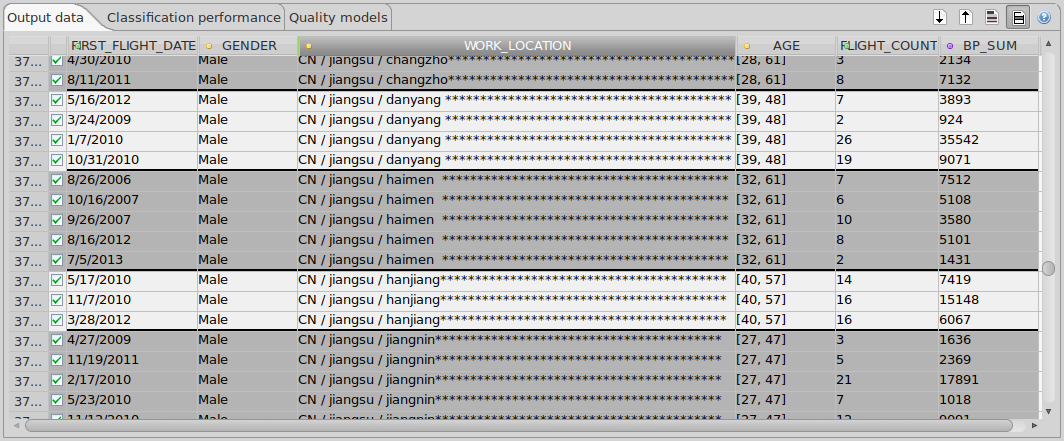
\includegraphics[width=\textwidth]{figures/classes.png}
\caption{Exemplary equivalence classes as found by ARX.}
\label{fig:classes}
\end{figure}

Fig.~\ref{fig:paths} shows the anonymization paths that ARX finds for $k=3$ and $k=50$, respectively. To achieve the same level of anonymity, either the gender attribute can be suppressed or the contained information about the work location can be reduced, resulting in the paths shown in Fig.~\ref{fig:paths}.

For different $k$, the paths don't show significant differences. However, aiming at the same level of anonymity, ARX has to suppress more information when selecting a lower $k$.

Fig.~\ref{fig:classes} shows an excerpt of an solution ARX finds for $k=3$. Some of the equivalence classes indeed assume the desired size of 3, while others are substantially larger.

\begin{figure}
\centering
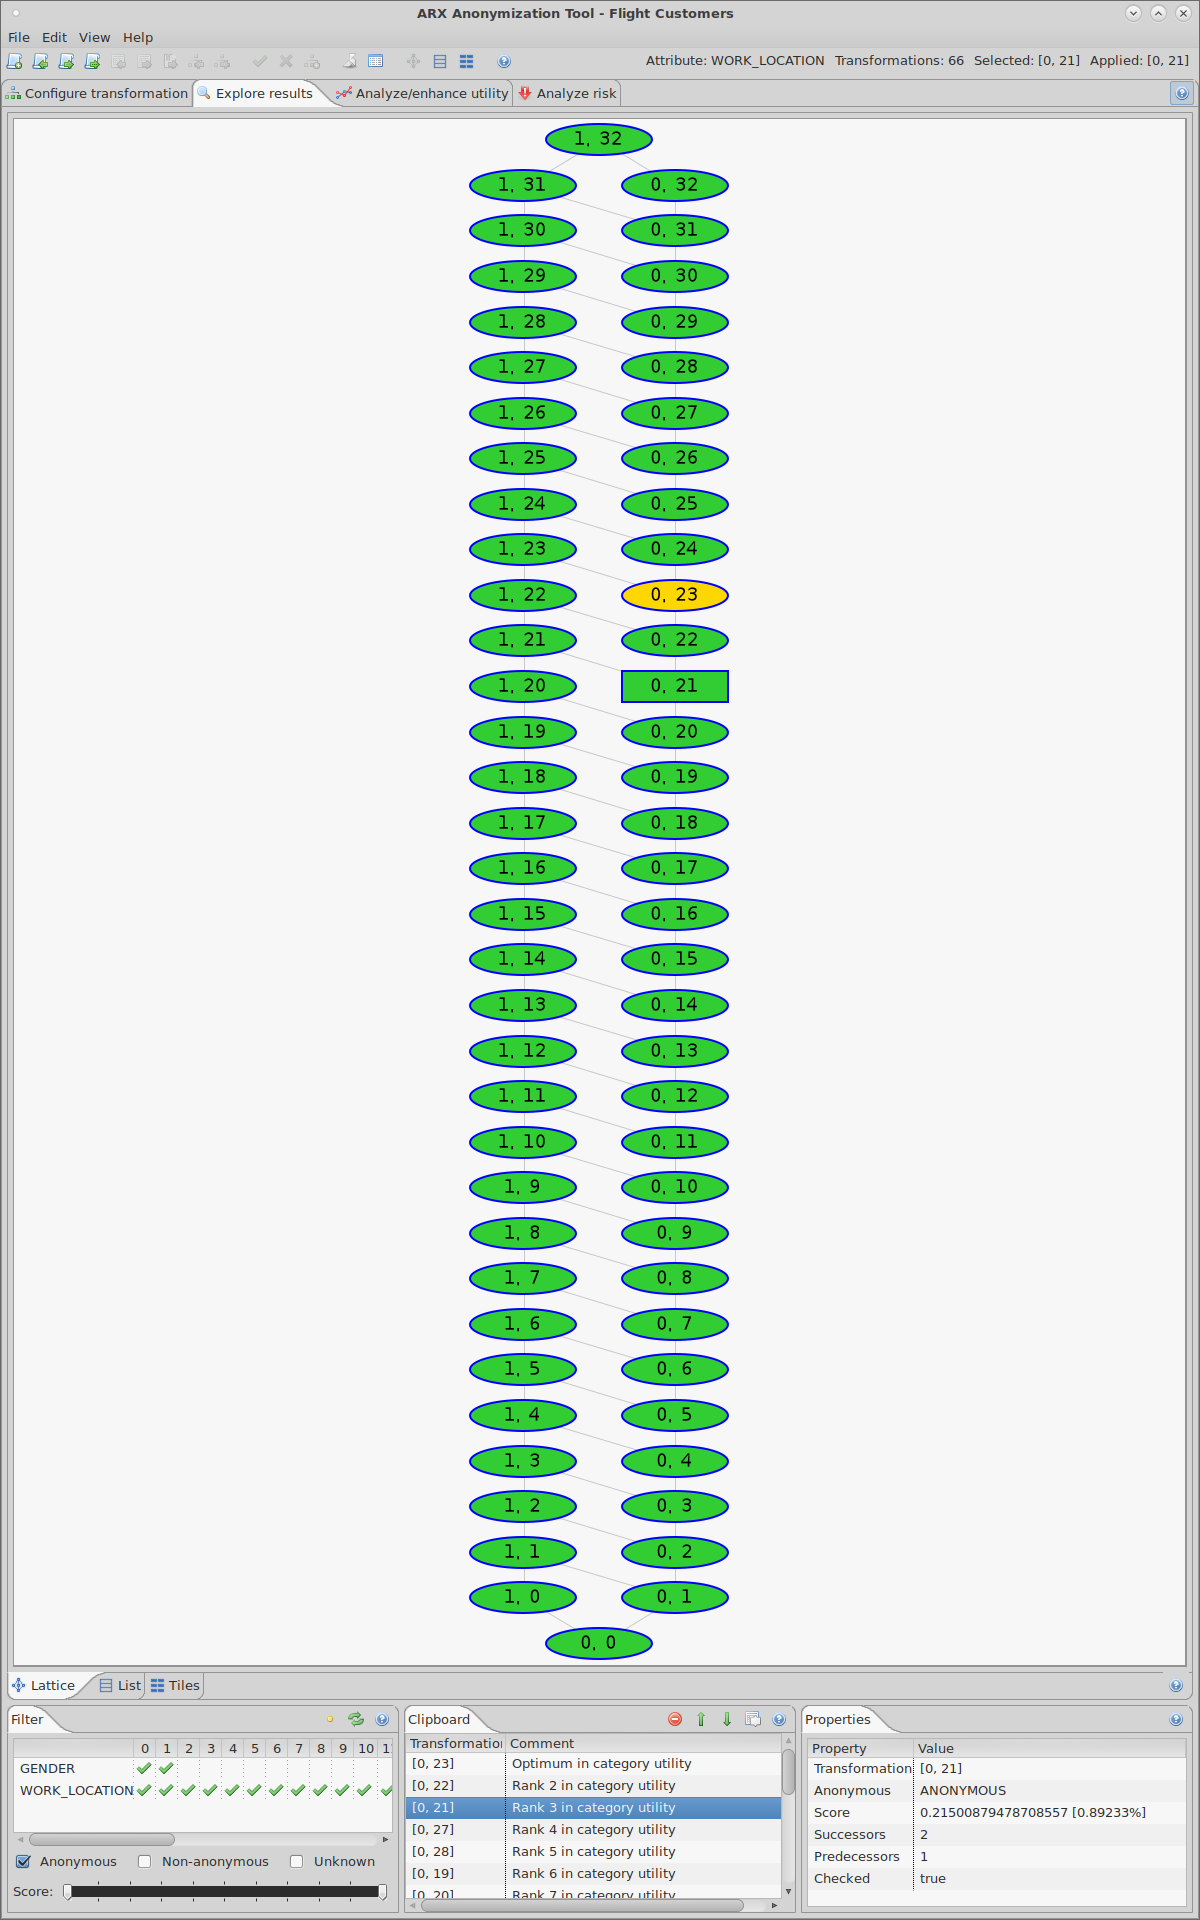
\includegraphics[trim=10cm 9cm 10cm 4.4cm, clip,width=0.4\textwidth]{figures/k=3_paths.png}
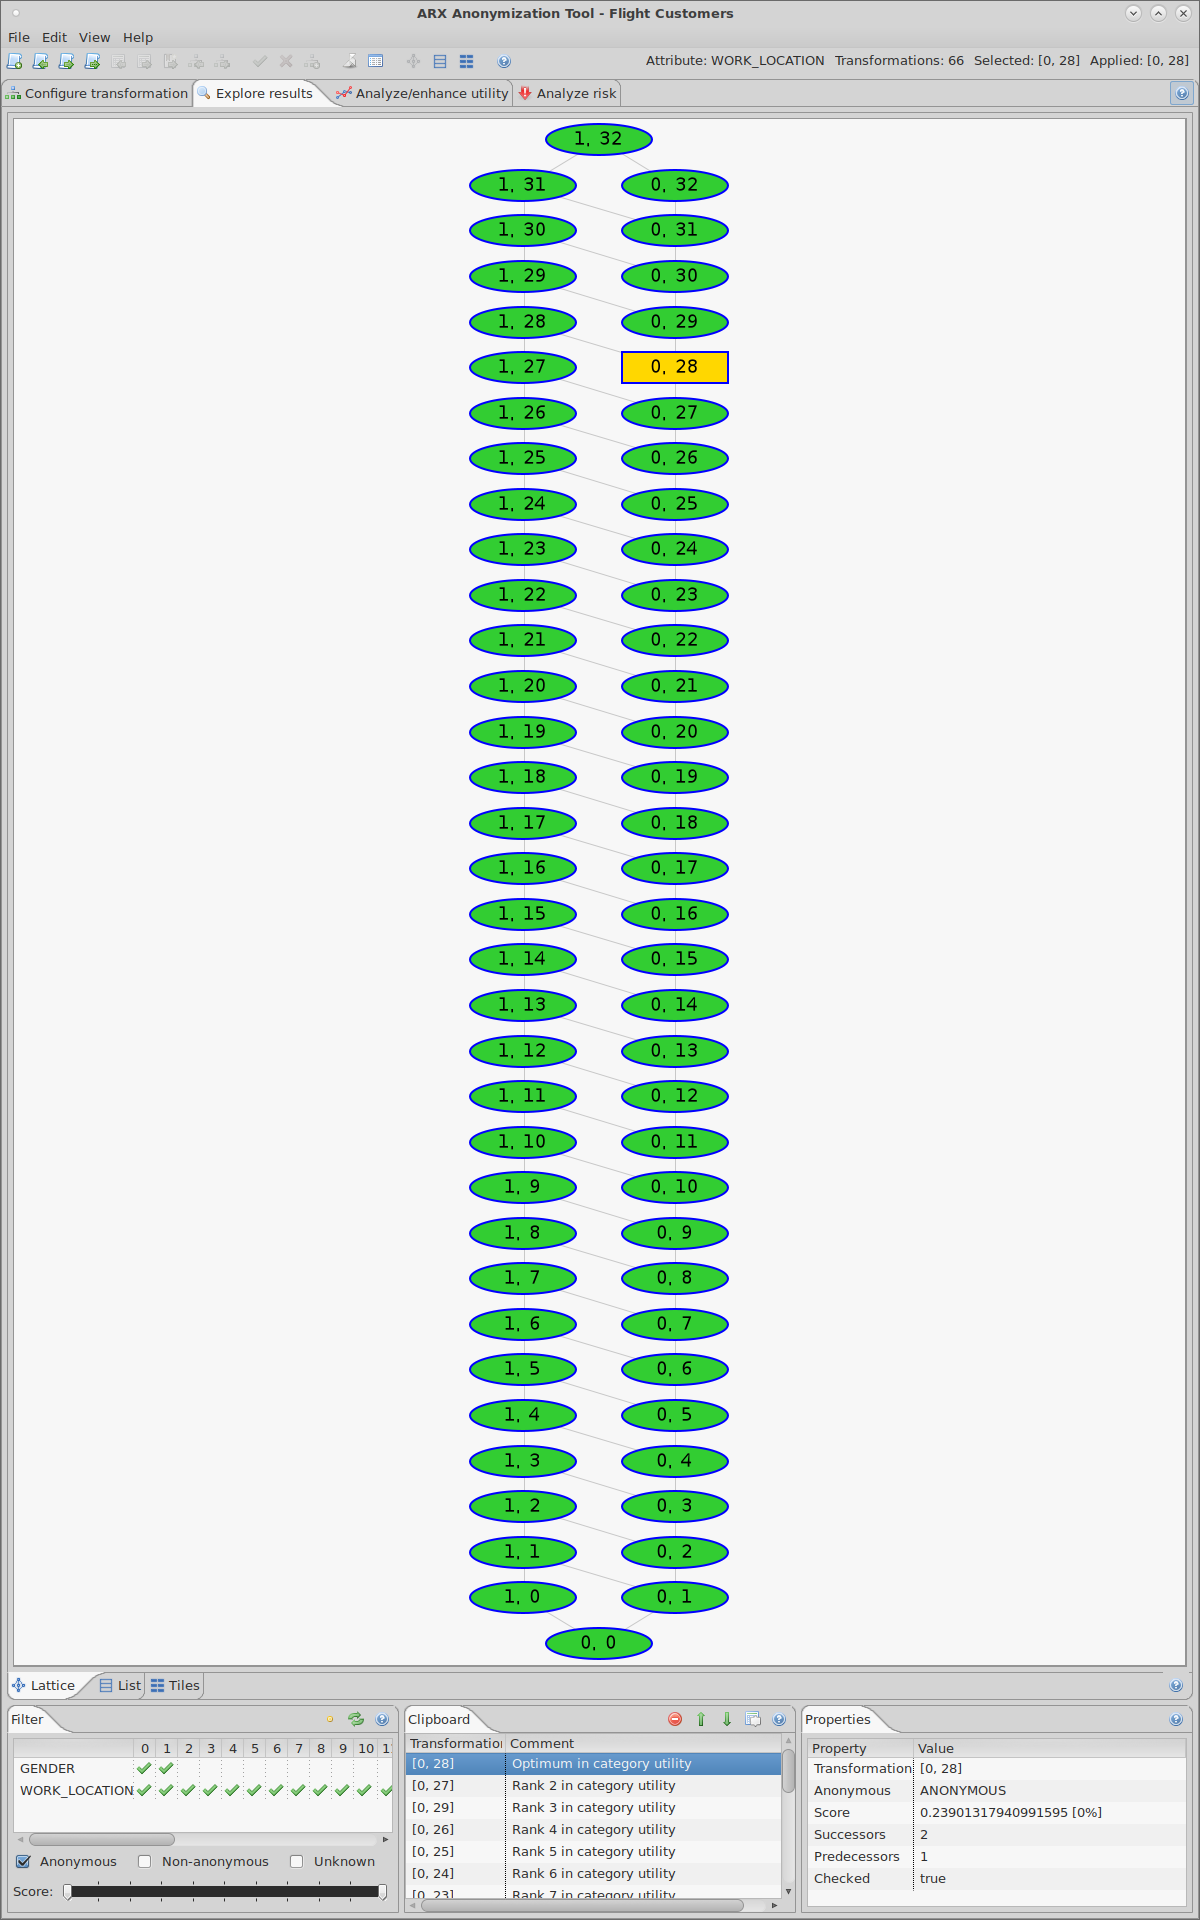
\includegraphics[trim=10cm 9cm 10cm 4.4cm, clip,width=0.4\textwidth]{figures/k=50_paths.png}
\caption{Anonymization paths for $k=3$ (left) and $k=50$ (right).}
\label{fig:paths}
\end{figure}


%%%%%%%%%%%%%%%%%%%%%%%%%%%%%%%%%%%%%%%%%%%%%%%
\end{document}
